\chapter{Hardware}
\label{cha:Hardware}

\todo{Einleitung}
\section{Der Raspberry Pi}
\label{sec:Raspberry}
Der \emph{Raspberry Pi} ist ein Einplatinencomputer, der 2012 von der \emph{Raspberry Pi Foundation} auf den Markt gebracht wurde.

\begin{figure}[h]
  \centering
     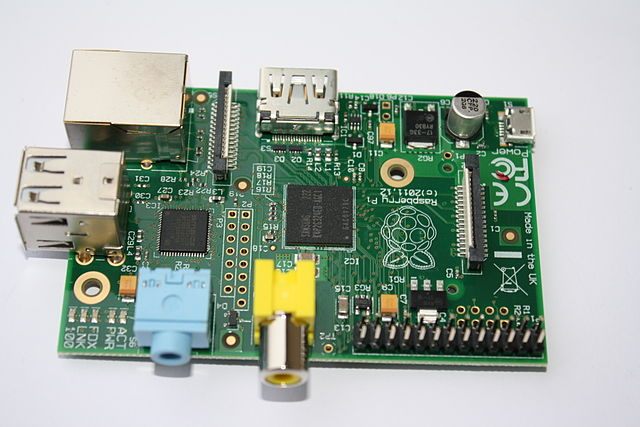
\includegraphics[width=0.8\textwidth]{figures/raspberry.jpg}
 \caption[Raspberry Pi - Modell B]{Raspberry Pi - Modell B\footnotemark}
  \label{fig:raspberry}
\end{figure}
\footnotetext{\cite{rasp_bild}}

\subsection{Geschichte}
\label{subsec:Geschichte}
Ursprünglich war der Raspberry Pi als günstiger Computer gedacht, um britischen Jugendlichen das Programmieren näher zu bringen. An der \emph{University of Cambridge} stellte man fest, dass die Vorkenntnisse von Studienanfängern immer geringer wurden, weil sie -- sowohl privat als auch in der Schule -- sich immer weniger mit der Funktionsweise von Computern und Programmen beschäftigen. Daher wollte man einen Computer entwickeln, mit dem die Jugendlichen experimentieren können.
\footcite{aboutraspberry}$^,$
\footcite[Geschichte]{wiki:raspberry}

Inzwischen wurden 3,8 Millionen Stück verkauft (Stand Oktober 2014\footcite{verkauf}) und 5 verschiedene Modelle entwickelt.

\subsection{Technische Daten}
\label{subsec:Technische Daten}
Die Technik in einem Raspberry Pi ist vergleichbar mit der eines Smartphones. Der Raspberry Pi hat eine \acrshort{cpu} mit \SI{700}{\glslink{Hertz}{\mega\hertz}}, welche auf bis zu \SI{1}{\glslink{Hertz}{\giga\hertz}} übertaktbar ist, und je nach Modell \SI{256}{} oder \SI{512}{\mega\byte} Arbeitsspeicher. Als Speicher für das Betriebssystem (verschiedene Linux-Distributionen stehen zur Auswahl) wird eine SD-Karte bzw. eine microSD-Karte verwendet.

Zur Stromversorgung genügt ein normales Handyladegerät mit Micro-USB-Anschluss und mindestens \SI{1}{\gls{Ampere}} Stromstärke, denn der Raspberry Pi verbaucht nur \SI{3.5}{Watt}\footcite{strom} (Modell B).

Zum Anschließen anderer Hardware gibt es zwei USB-Anschlüsse und 26 \gls{gpio}-Pins.

\section{Sensoren}
\label{sec:Sensoren}

Zur Messung der Umweltdaten werden folgende Sensoren verwendet:
\begin{itemize}
\item 4 Temperatursensoren \emph{DS18B20} (\ref{subsec:Temperatur})
\item Luftfeuchtesensor \emph{DHT22} (\ref{subsec:Luftfeuchtigkeit})
\item Luftdrucksensor \emph{BMP085} (\ref{subsec:Luftdruck})
\item Luftqualitätssensor \emph{VOLTCRAFT CO-20} (\ref{subsec:Luftqualitat})
\item CPU-Temperatur des Raspberry Pi
\end{itemize}
\subsection{Temperatur}
\label{subsec:Temperatur}

Mithilfe von 4 Sensoren des Typs \emph{DS18B20} werden die Innentemperatur, die Gehäusetemperatur und die Bodentemperatur (Außen) gemessen. Diese haben eine Messgenauigkeit von \SI{\pm 0.5}{\degreeCelsius}  und einen Messbereich von \SI{-10}{\degreeCelsius}  bis \SI{+85}{\degreeCelsius}. \footcite[20]{temp}

\begin{figure}[h]
  \centering
     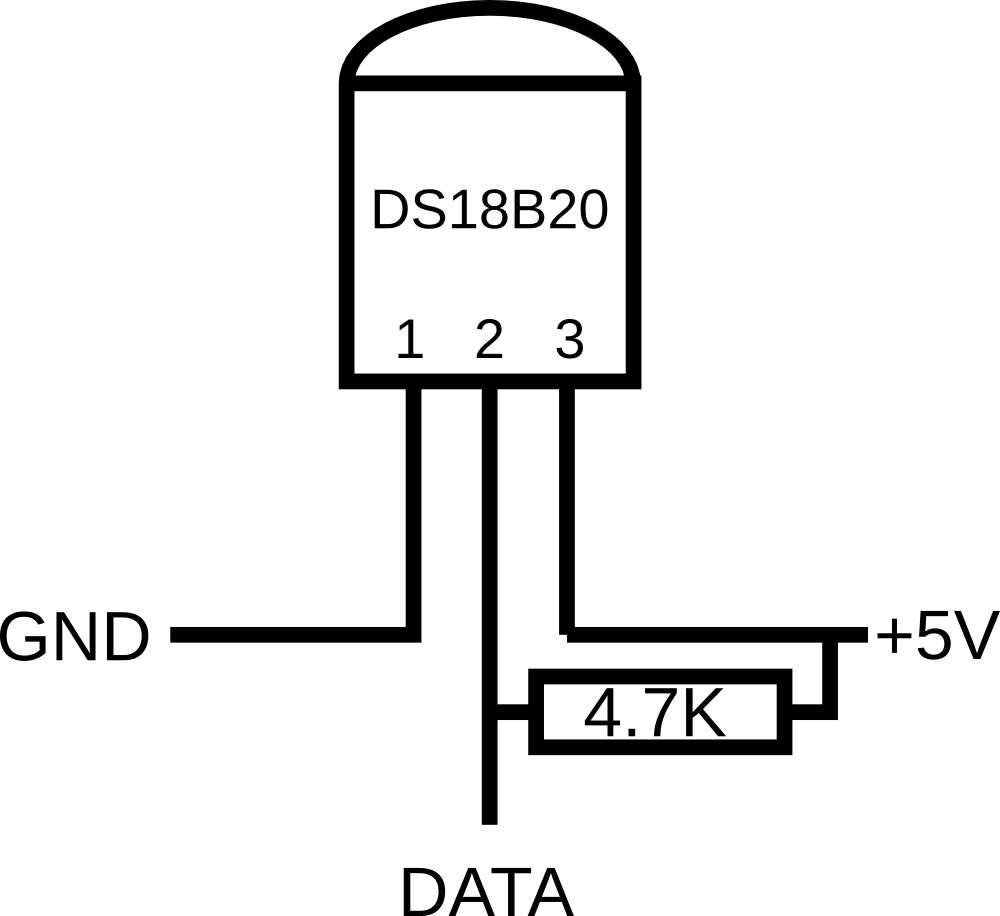
\includegraphics[width=0.4\textwidth]{figures/temp_pin.png}
  \caption{Pinbelegung des DS18B20 (eigenes Werk)}
  \label{fig:temp_pin}
\end{figure}

Der Sensor wird mithilfe von einem \gls{1-Wire}-\gls{Bus} ausgelesen. Hierbei benötigt man (außer für die Stromversorgung mit \SI{5}{\gls{Volt}} nur ein Kabel, auf dem die Daten übertragen werden.\footcite{1-wire} Zusätzlich wird ein \SI{4.7}{\kilo\glslink{Ohm}{\ohm}} Widerstand zwischen dem Pin für Daten und dem Pin für \SI[retain-explicit-plus]{+5}{\glslink{Volt}{\volt}} benötigt. (siehe Abb. \ref{fig:temp_pin})
Ein weiterer Vorteil von 1-Wire ist, dass nahezu beliebig viele Sensoren auf einem Datenkabel parallel geschaltet werden können.

Die Messdaten des \emph{DS18B20} können auf dem Raspberry Pi sehr einfach ausgelesen werden, weil dies von einem Linux-\gls{Kernelmodul} erledigt wird. Um die Temperatur zu erhalten, muss  nur eine virtuelle Datei ausgelesen werden, welche das Messergebnis in tausendstel Grad Celsius enthält. (Siehe Abbildung \ref{fig:temp_screenshot})

\begin{figure}[h]
  \centering
     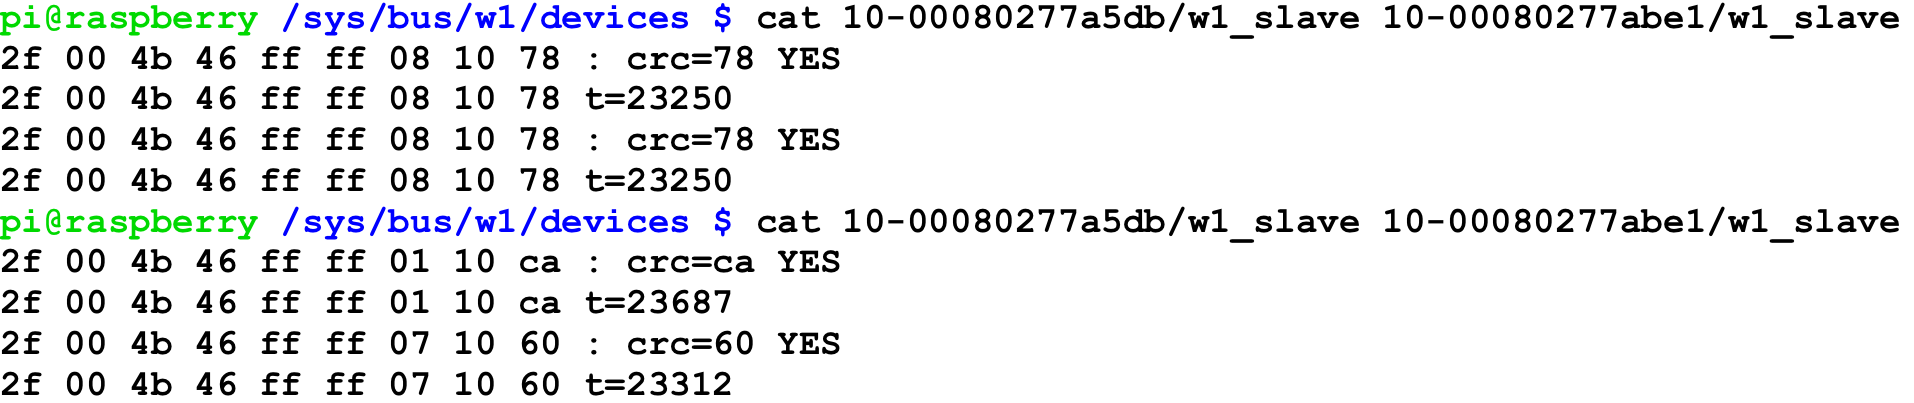
\includegraphics[width=\textwidth]{figures/temp_screenshot.png}
  \caption{Die erste erfolgreiche Messung (eigenes Werk)}
  \label{fig:temp_screenshot}
\end{figure}

\subsection{Luftfeuchtigkeit}
\label{subsec:Luftfeuchtigkeit}

Zum Messen der Luftfeuchtigkeit der Außenluft wird der \emph{DHT22} verwendet. Dieser kann auch die Temperatur messen. Die Messgenauigkeit beträgt \SI{\pm 0.5}{\degreeCelsius} und \SI{\pm 2}{\% .relative.Luftfeuchte}.\footcite{DHT22}
Wie der \emph{DS18B20} (\ref{subsec:Temperatur}) benötigt der Luftfeuchtigkeitssensor zusätzlich zur Stromversorgung nur ein Kabel zur Datenübertragung. Es können jedoch nicht mehrere Sensoren parallel geschaltet werden. \footcite[Wiring]{DHT}

\begin{figure}
  \centering
     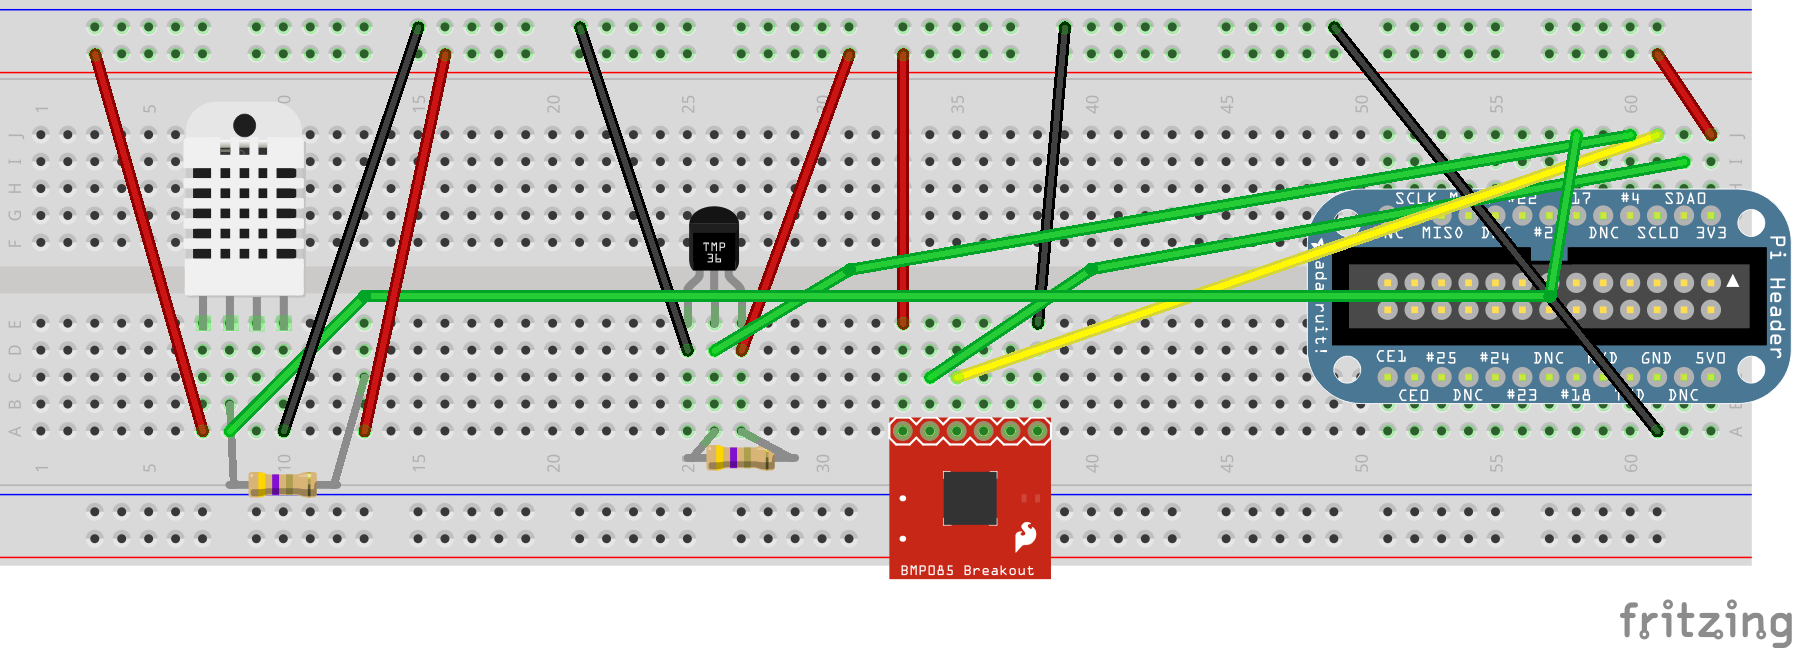
\includegraphics[width=\textwidth]{figures/steckbrett.png}
  \caption{Anschlussskizze von \emph{DS18B20} (Mitte; \ref{subsec:Temperatur}), \emph{DHT22} (Links; \ref{subsec:Luftfeuchtigkeit}) und \emph{BMP085} (Rechts; \ref{subsec:Luftdruck}) (eigenes Werk)}
  \label{fig:steckbrett}
\end{figure}

Die Daten des Sensors werden von einem \gls{C}-Programm von Adafruit ausgelesen.
\footcite[Software Install]{DHT}

\subsection{Luftdruck}
\label{subsec:Luftdruck}

Der \emph{BMP085} ist der präziseste Sensor. Er wird zum Messen des Luftdruckes und der Außentemperatur verwendet und hat dabei eine Genauigkeit von \SI{\pm 1.0}{\hecto\glslink{Pascal}{\pascal}} und \SI{0.5}{\degreeCelsius} bei \SI{25}{\degreeCelsius}\footcite[6]{BMP085}

Die Messdaten überträgt der Sensor über einen \gls{I2C}-\glslink{Bus}{Bus}. Dabei werden (zusätzlich zur Stromversorgung) \textbf{zwei} Kabel zur Datenübertragung benötigt.
Über eines (in Abbildung \ref{fig:steckbrett} gelb) schickt der Raspberry Pi dem Sensor die Taktfrequenz, in der er die Daten übertragen soll, und im anderen (grün) werden die eigentlichen Daten übertragen.
\footcite[Hooking Everything Up]{bmp058_adafruit}

Auch hier werden die Daten von einem Programm von Adafruit ausgelesen. \footcite[Using the Adafruit BMP Python Library (Updated)]{bmp058_adafruit}

\subsection{Luftqualität}
\label{subsec:Luftqualitat}
Der letzte Sensor, der hinzugekommen ist, ist der \emph{VOLTCRAFT CO-20}. Da CO\textsubscript{2}-Sensoren und andere genaue Luftqualitätssensoren teuer sind, habe ich mich für einen einfachen \acrshort{voc}-Sensor entschieden. Dieser misst die Menge an \emph{Flüchtigen organischen Verbindungen} in der Luft. Dies sind Stoffe, die schon bei niedrigen Temperaturen verdampfen. Sie können von verschiedensten Quellen stammen (\zB: Benzindämpfe, Tabakrauch, Lacke)\footcite[41\psqq]{innenraum} und von leichten Kopfschmerzen und Konzentrationsstörungen bis zu bleibenden Gesundheitsschäden führen.\footcite[Gesundheitliche Wirkung]{VOC}

Der Sensor gibt einen Wert an, der die relative Verschlechterung seit dem Einschalten angibt. Hierbei steht 450 für die anfängliche Qualität ist und ein höherer Wert für eine schlechtere Luftqualität.
Da der \emph{VOLTCRAFT CO-20} jedoch nicht mehr erhältlich ist, verwende ich den baugleichen \emph{Raumluftfühler} von Velux.\footcite{Velux}

\begin{figure}[h]
  \centering
     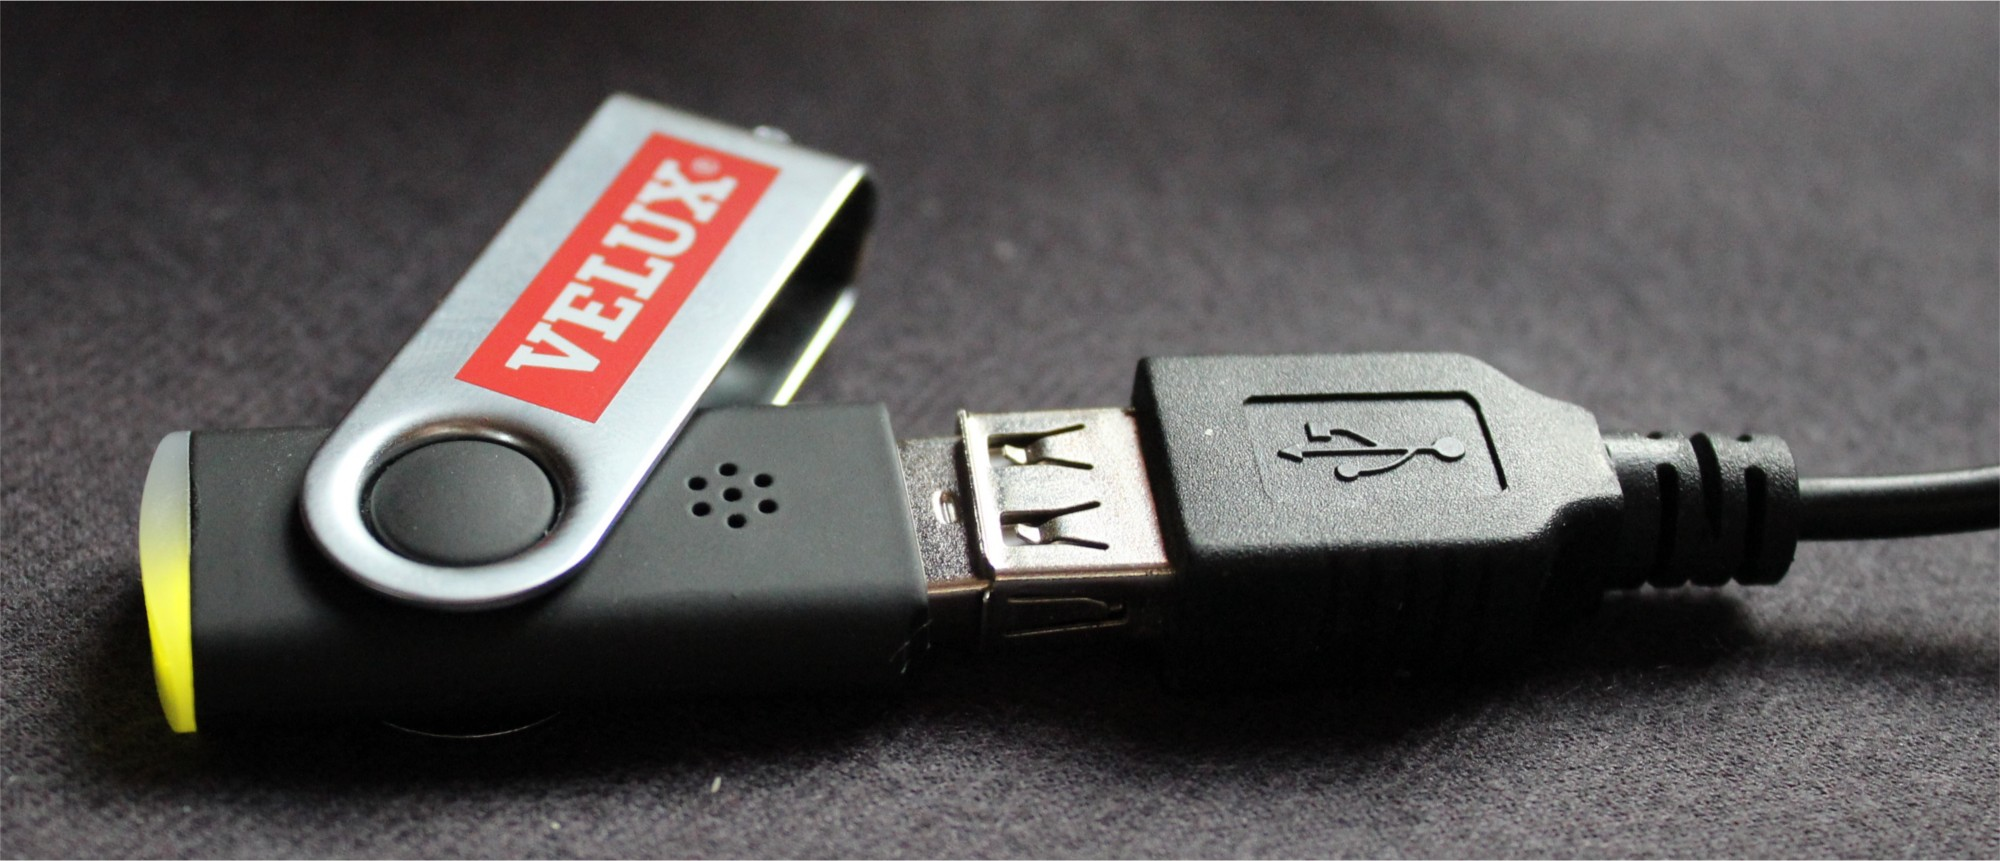
\includegraphics[width=\textwidth]{figures/velux.jpg}
  \caption{Velux Raumluftfühler (eigenes Werk)}
  \label{fig:velux}
\end{figure}

Der Sensor wird über USB an den Raspberry Pi angeschlossen. Um die Daten unter Linux auszulesen, wird das Programm \emph{usb-sensors-linux} verwendet.\footcite{usb-sensors-linux}

\section{Display}
\label{sec:Display}

\begin{figure}[h]
  \centering
     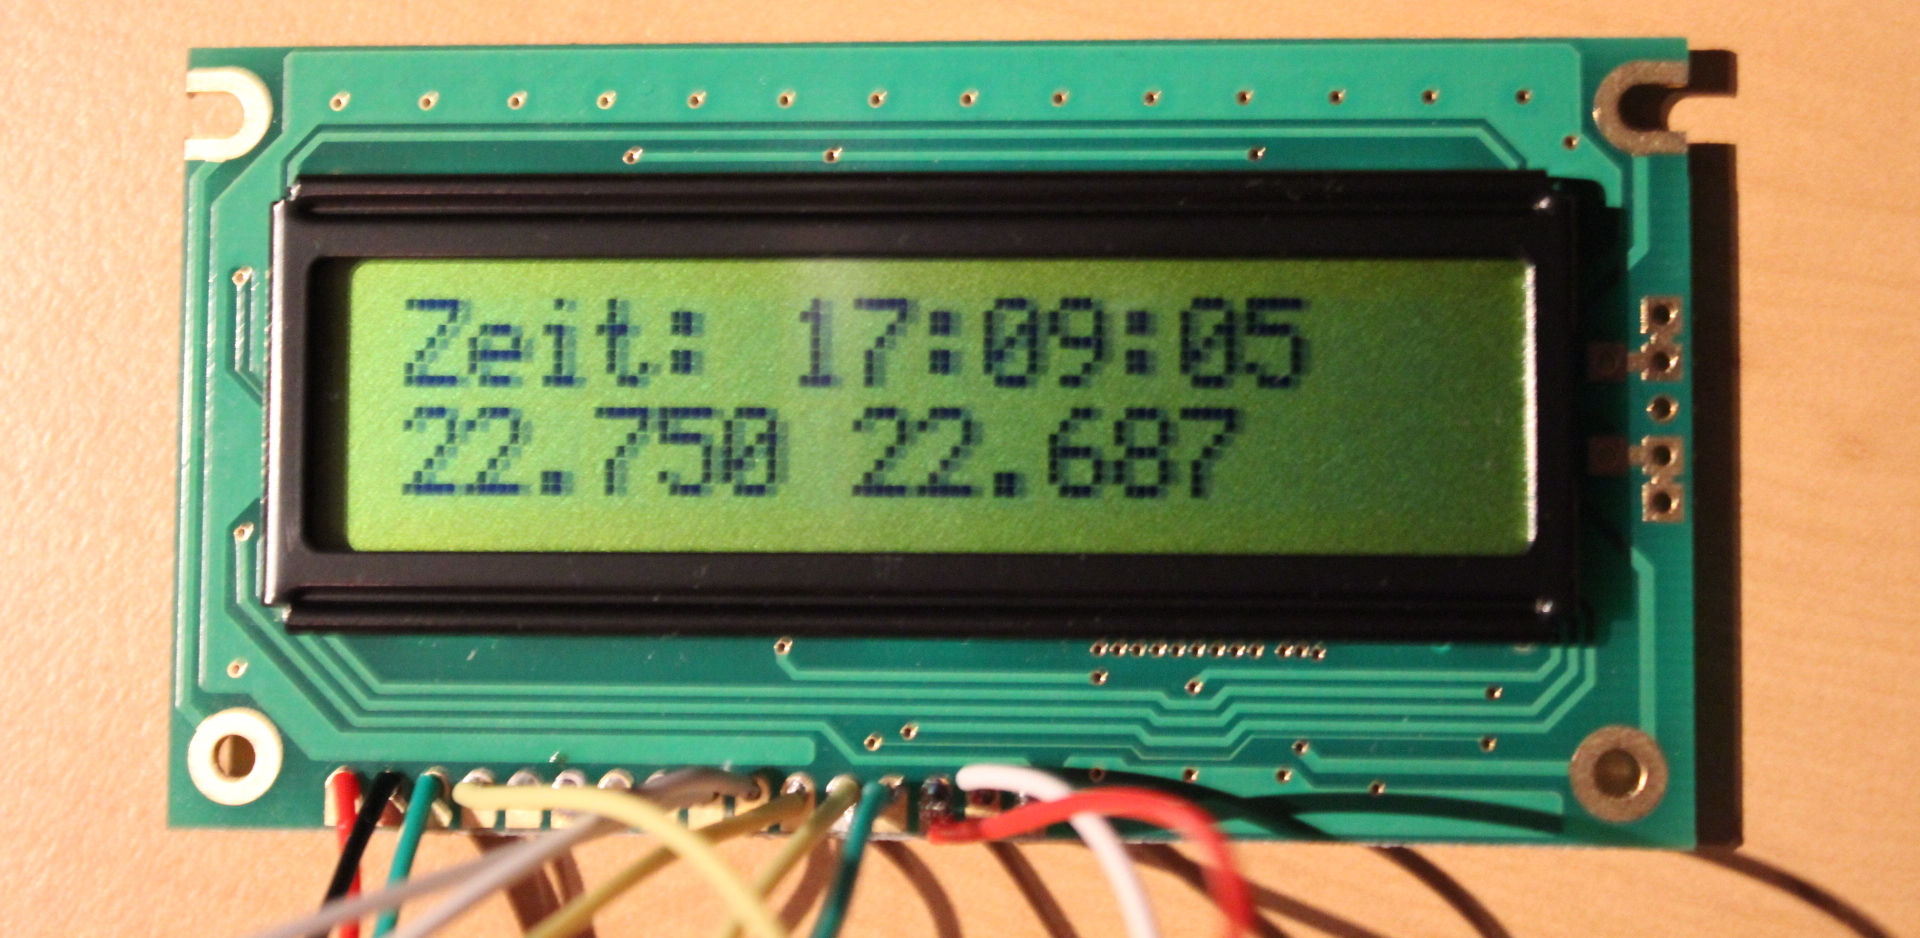
\includegraphics[width=0.9\textwidth]{figures/erstes_display.jpg}
  \caption{Erstes Display (eigenes Werk)}
  \label{fig:erstes_display}
\end{figure}

Damit nicht immer ein Computer benötigt wird, um die aktuellen Messwerte zu erfahren, verwende ich ein Display, welches diese anzeigt. Ursprünglich habe ich ein 16x2 Zeichen Display von \emph{Conrad Electronic} verwendet.\footcite{conrad_datenblatt}
Dieses wird nach der Anleitung von \emph{www.schnatterente.net}\footcite{schnatterente} angeschlossen.

Da jedoch fix angelötete Kabel unflexibel sind, bin ich auf ein Display von \emph{Pollin.de}\footcite{display_pollin} umgestiegen, welches mit einer Steckverbindung angeschlossen wird.

\section{Anschluss}
\label{sec:Anschluss}
\todo[inline]{Kapitel über Gehäuse, Platinen, Zusammenbau}